\subsection{Formulace problému}
\label{subsec:definice_problemu}
V předešlé sekci byl popsán proces předzpracování dat, jehož výsledkem je nová
multidimenzionální množina segmentovaných fyziologických signálů $\mathcal{F}$.
Dimenze této množiny je rovna počtu snímaných signálů, lze tedy dál hovořit jako
o kanálech $c$. Vybraný segment z kanálu $c$ reprezentuje časovou řadu, jejiž
každý vzorek je zachycen v určitém čase $t$, a představuje průběh fyziologické
události (\gls{NPF} událost).

V rámci jednotlivých pozorovaných fyziologických událostí $X^i$, lze modelovat
časově kauzální vztahy, které lze díky Grangerově kauzalitě (viz
sekce~\ref{subsec:granger}) matematicky popsat unikátním orientovaným grafem
$G=(V,E)$ -- definovanou uspořádanou množinou vrcholů a hran. Tím je umožněno
temporální kódování specifického příčinného kognitivního stavu pro konkrétní
segment vybraného kanálu $c$. Nelze však předpokládat, že je tak zachycena
veškerá komplexní dynamika, která je ve biosignálech přítomna, včetně toho, že
nemusí být plně zachyceny interakce napříč kanály $c$.

Tento problém je kompenzován použitím vícerozměrných časoprostorových vzorů
(\gls{GAF}, Gramian Angular Fields) odvozených z Gramových matic. Tyto vzory
zachycují určitý druh temporální i prostorové korelace v rámci fyziologických
událostí. V následujících sekcích je dále popsána tvorba zmíněných příznaků
společně s jejich aplikací v rámci strojového učení.

\subsection{Tvorba kauzálních vícerozměrných matic}
\label{subsec:kauzalni_matice}
Pro zachycení časově kauzálních relací v použitých biosignálech byl zvolen
přístup Kopula-Granger s Lasso ($\ell_1$) regularizací, který kombinuje koncept
Grangerovy kauzality s teorií kopulí. Zmíněné přístupy spadají do oblasti
statistických metod, a proto jsou dále jednotlivé popsány v
sekci~\ref{sec:statisticke_metody}.

Vytvoření kauzální matice ja založeno na použití fyziologické události $X^i$
definované v minulé sekci, ze které lze uplatněním Kopula-Granger metody získat
robustní odhad koeficientů vektorů $\beta_i$ pro test Grangerovy kauzality
využitím regresní úlohy. K tomu je ale potřeba vyřešit následující optimalizační
problém~\cite{Schindler2013,Guy2016}:
\begin{equation}
    \min _{\beta_i} \sum_{l=L+1}^T\left|X_t^i-\sum_{j=1}^p\left(X_{t, \text {lag}}^j\right) \cdot\left(\beta_i^j\right)^{\prime}\right|^2+\lambda\left\|\beta_i\right\|_1,
\end{equation}
kde $\lambda$ je penalizační parametr ovlivňující řídkost vektoru $\beta_i$, $L$
je maximální časové zpoždění (lag) a ${X}_{t, \text {lag}}^j$ jsou předchozí
hodnoty řady $X^j$ v čase $[t - L, t - 1]$. Podle definice Kopula-Granger
modelu~\cite{Schindler2013,Guy2016} lze dále uplatnit faktorizaci na základě
modelu vektorové autoregrese (\gls{VAR}) s koeficienty $B = {{\beta}_{i}^j}$
následovně:
\begin{equation}
    p_Z(z)=\mathcal{N}(z(1, \ldots, L)) \times \prod_{j=1}^n \prod_{t=L+1}^T p_{\mathcal{N}}\left(z_j(t) ; \sum_{t=1}^n \beta_{i, j}^T z_i^{t, \text {lag}}, \sigma_j\right)
\end{equation}
kde $p_{\mathcal{N}}(z ; \mu, \sigma)$ je Gaussova funkce se střední hodnotou
$\mu$ a rozptylem $\sigma^2$, $z_i^{t, \text {lag}}$ jsou předchozí hodnoty
$z_i$ do času $t$ a ${\beta}_{i}^j$ je vektor koeficientů modelujících vliv
časové řady $z_j$ na cílovou časovou řadu. Kauzalita je tedy definována časovou
řadou $z_j$, jež je příčinou $z_i$ pokud je alespoň jedna hodnota vektoru
${\beta}_{i}^j$ nenulová ve smyslu statistické významnosti
(viz~\ref{subsec:granger}).

\begin{figure}[h]
    \begin{center}
        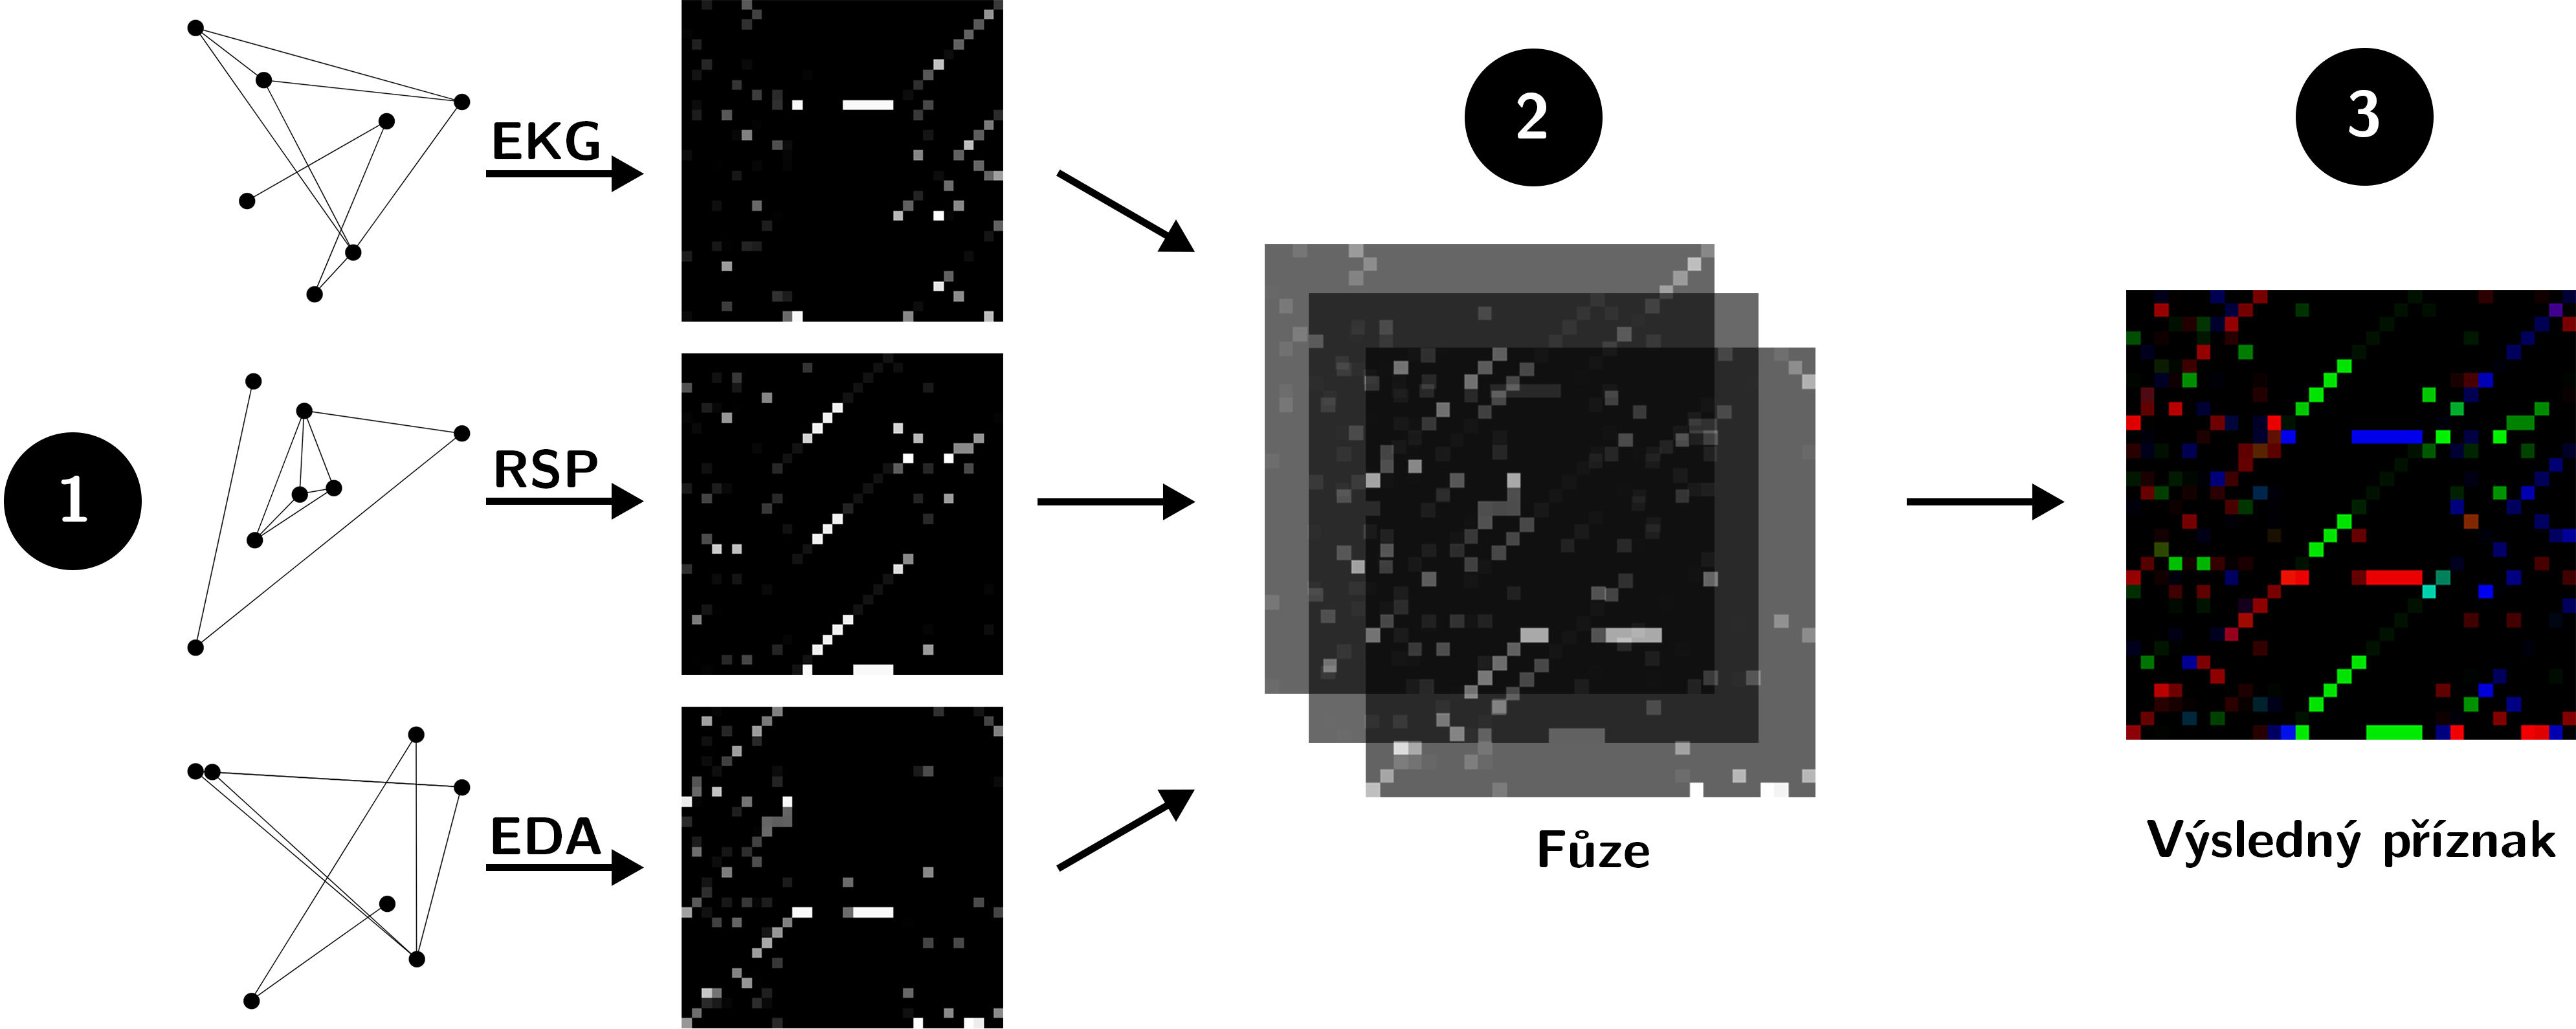
\includegraphics[width=1\linewidth]{figures/GCN}
        \caption{Diagram tvorby kauzálních vícerozměrných matic. 1) Aplikace
            Kopula-Granger metody pro vybraný segment všech kanálů $c$. 2) Kombinace
            výsledných kauzálních matic do jednoho trojrozměrného pole. 3) Výsledný
            příznak ve smyslu RGB obrázku}
        \label{fig:GCN}
    \end{center}
\end{figure}

Kopula-Granger metodu lze primárně shrnout do dvou kroků: odhadnutí marginální
distribuční funkce vybrané časové řady $X^i$ jako $\hat{F_i}$ a mapování
pozorovaných hodnot fyziologické události v čase $t$ do kopula prostoru jako
$Z_{i}^t=\Phi^{-1}\left(\hat{F}_i\left(X_{t}^i\right)\right)$, kde $\Phi$ je
kumulativní distribuční funkce (\gls{CDF}) Gaussova rozdělení. V neposlední řadě
lze konstruovat temporální kauzální graf analýzou relací mezi $Z_{i}^t$. Pro
účely tvorby grafického řešení v podobě kauzální matice $T \times T$ obsahující
odhady koeficientů $\hat{\beta}_i$ byla adaptována regularizovaná regrese
podle~\cite{Bahdori2012}. Nechť vybraná fyziologická událost $X^i = \{x_t^i : t
= 0,...,T\}$, poté lze získat koeficienty následovně:
\begin{equation}
    \hat{\beta}_i(\lambda)=\arg \min _{\beta_i}\left(\sum_{t=1}^T\left\|x_i^t-X_{t, L}^{lag} \beta_i\right\|^2+\lambda\left\|\beta_i\right\|_1\right)
\end{equation}
kde $X_{lag}^{t, L}$ reprezentuje spojený vektor všech zpožděných pozorování s
maximálním zpožděním $L$ až do času $t$. Tvorba kauzálních matic byla
realizována v programovém prostředí Matlab s využitím knihovny
\textit{GLMNET}\footnote{\url{https://hastie.su.domains/glmnet_matlab}}, která
umožňuje specifikovat různé typy regresních modelů. Hodnota časového zpoždění
byla určena na základě Akaikeho informačního kritéria (\gls{AIC}) jako $L = 4$.
Během každého výpočtu bylo pomocí zmíněné knihovny realizováno i automatické
ladění hodnot penalizačního parametru $\lambda \in m_i$, kde $m_i = 10^{a +
(i-1)d}$ pro $i = {1, 2, ..., 6}$ a $d = \frac{b-a}{n-1}$. Hodnoty $a$ a $b$
byly nastaveny na -3 a 2.

\subsection{Konstrukce časoprostorových polí}
\label{subsec:gadf}
Bylo realizováno mapování segmentů všech kanálů $c$ do prostorové domény
(\gls{GAF}), jež zachovává časové závislosti. Wang and Oates~\cite{Wang2015}
představili koncept této metody transformace časové řady do 2D obrazu v roce
2015. Vzhledem k dříve definované fyziologické události, tedy vybrané časové
řadě $X^i = \{x_1^i, x_2^i, \dots, x_t^i\}$ z kanálu $c$ zahrnuje konstrukce
\gls{GAF} nejdříve normalizaci na interval $[-1; 1]$:
\begin{equation}
    \tilde{x}_t=\frac{\left(x_t-\max (X^i)+\left(x_t-\min (X^i)\right)\right.}{\max (X^i)-\min (X^i)}
\end{equation}

\begin{figure}[h]
    \begin{center}
        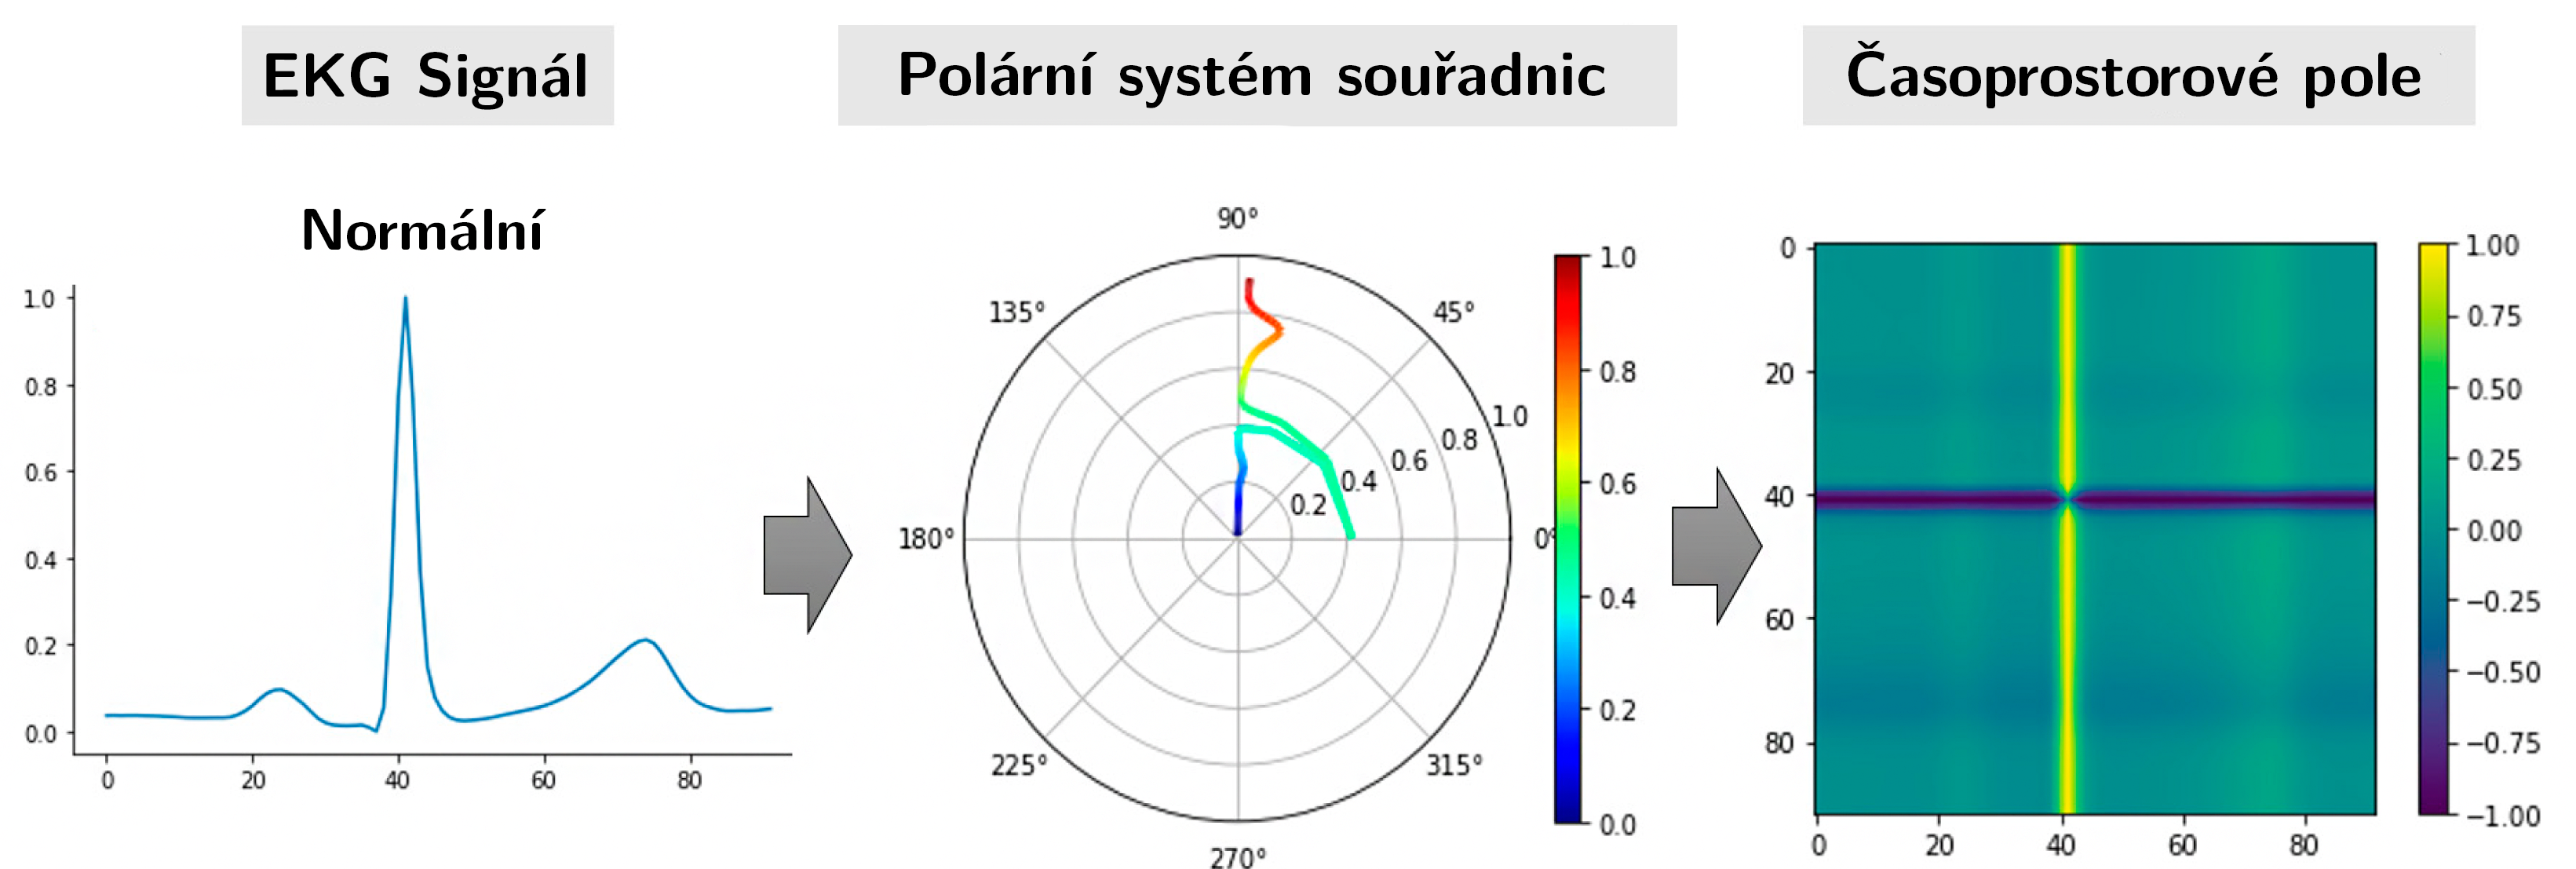
\includegraphics[width=1\linewidth]{figures/polar}
        \caption{Ukázka \gls{GAF} mapování na EKG segmentu}
        \label{fig:polar}
    \end{center}
\end{figure}

Dále jsou normalizovaná data časové řady převedeny do polárních souřadnic
výpočtem úhlové složky $\theta_i$ a radiální složky $r_i$ pro každý vzorek
$\tilde{x}_t$:
\begin{equation}
    \begin{cases}
        \theta_i = \arccos(\tilde{x}_t), & -1 \leq \tilde{x}_t \leq 1, \tilde{x}_t \in \tilde{X^i} \\
        r_i = \frac{t}{N},               & t \in N
    \end{cases}
\end{equation}
kde $t$ je časová značka vzorku fyziologické události a $N$ je konstantní faktor
pro regulaci rozpětí polárního souřadného systému. Jinými slovy, časová značka
představuje poloměr a arkus kosinus hodnoty časové řady úhel. Lze zde hovořit o
bijektivní transformaci, jež zachovává časovou závislost pomocí souřadnice $r$.

Po transformaci přeškálované časové řady do polárního souřadnicového systému lze
využít úhlovou perspektivu, v tomto případě s ohledem na trigonometrický rozdíl
mezi jednotlivými body (\gls{GADF}, Gramian angular field difference), k
identifikaci temporální korelace v rámci různých časových intervalů:
\begin{equation}
    GADF = \left[\sin \left(\phi_i-\phi_j\right)\right]
\end{equation}

\begin{figure}[h]
    \begin{center}
        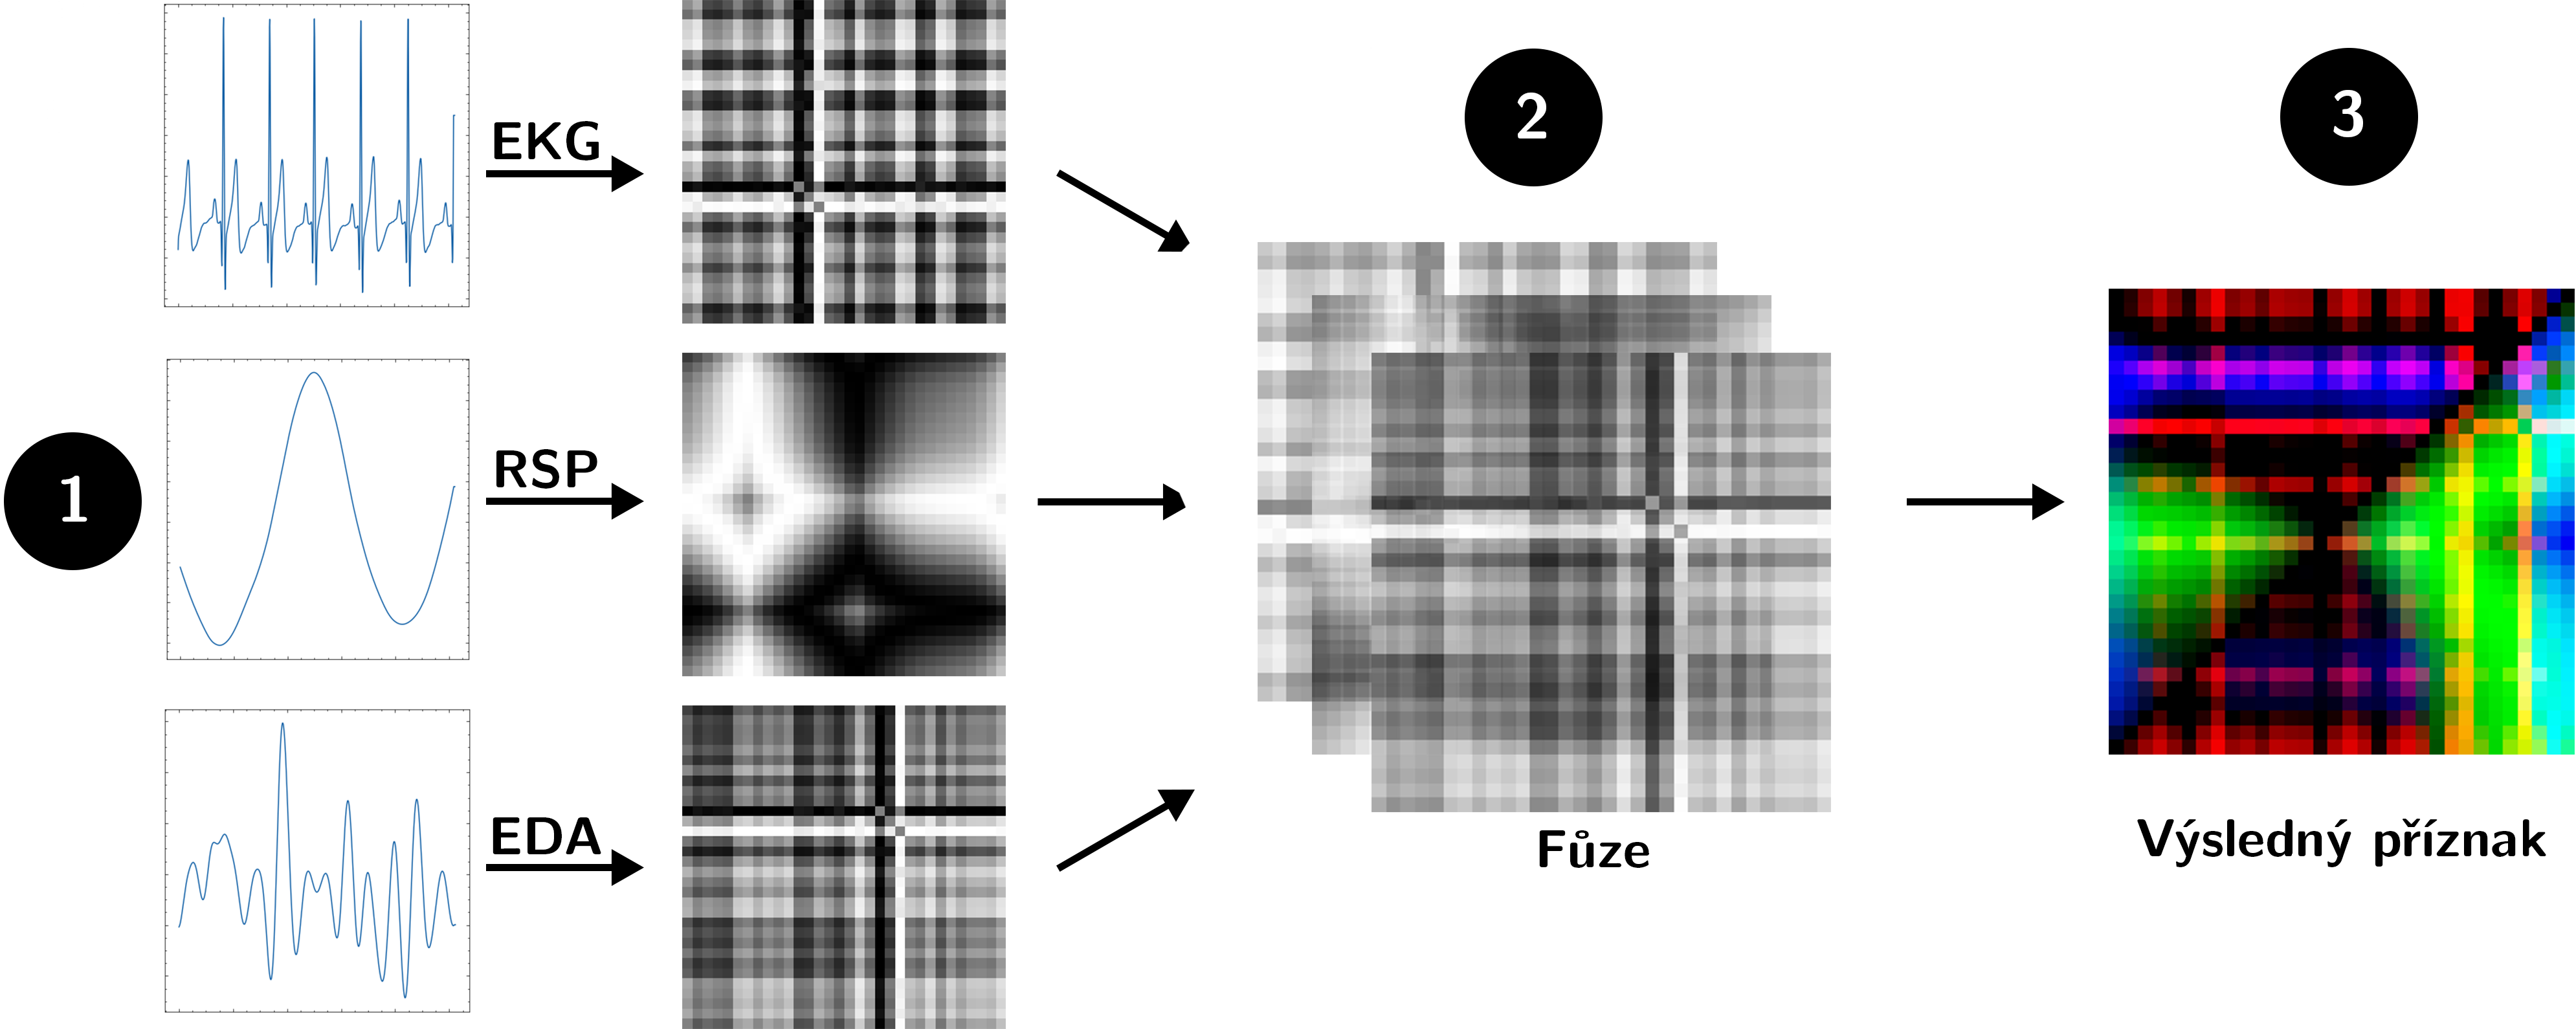
\includegraphics[width=1\linewidth]{figures/GADF}
        \caption{Diagram tvorby časoprostorových vzorů. 1) Aplikace GAF mapování
            pro vybraný segment všech kanálů $c$. 2) Kombinace výsledných polí
            do jednoho trojrozměrného pole. 3) Výsledný příznak kódující
            temporální korelace fyziologické události v prostorové doméně}
        \label{fig:gadf}
    \end{center}
\end{figure}

Ve výsledku je tedy časoprostorový vzor definován následující $T \times T$
maticí, která je kvazi-Gramovou maticí:
\begin{equation}
    GADF = \left[\begin{array}{cccc}
            \sin \left(\phi_1-\phi_1\right) & \sin \left(\phi_1-\phi_2\right) & \cdots & \sin \left(\phi_1-\phi_n\right) \\
            \sin \left(\phi_2-\phi_1\right) & \sin \left(\phi_2-\phi_2\right) & \cdots & \sin \left(\phi_2-\phi_n\right) \\
            \vdots                          & \vdots                          & \ddots & \vdots                          \\
            \sin \left(\phi_n-\phi_1\right) & \sin \left(\phi_n-\phi_2\right) & \cdots & \sin \left(\phi_n-\phi_n\right)
        \end{array}\right]
\end{equation}
kde každý prvek odpovídá sinové funkci úhlového sinusového rozdílu v různých
časových bodech. Výpočet a tvorba těchto příznaků, časoprostorových vzorů, byla
implementována v programovacím jazyce Python.

\subsection{Kapsulární neuronová síť}
\label{subsec:kapsularni_sit}
Pro potřeby realizace úloh klasifikace (resp. hodnocení kognitivní zátěže), byla
navržena architektura kapsulární neuronové sítě postavená na řešení, které
představili Mazzia et al.~\cite{Mazzia2021}, \textit{Efficient-CapsNet}.
Celkovou architekturu lze vidět na obrázku~\ref{fig:architektura}.

\begin{figure}[h]
    \begin{center}
        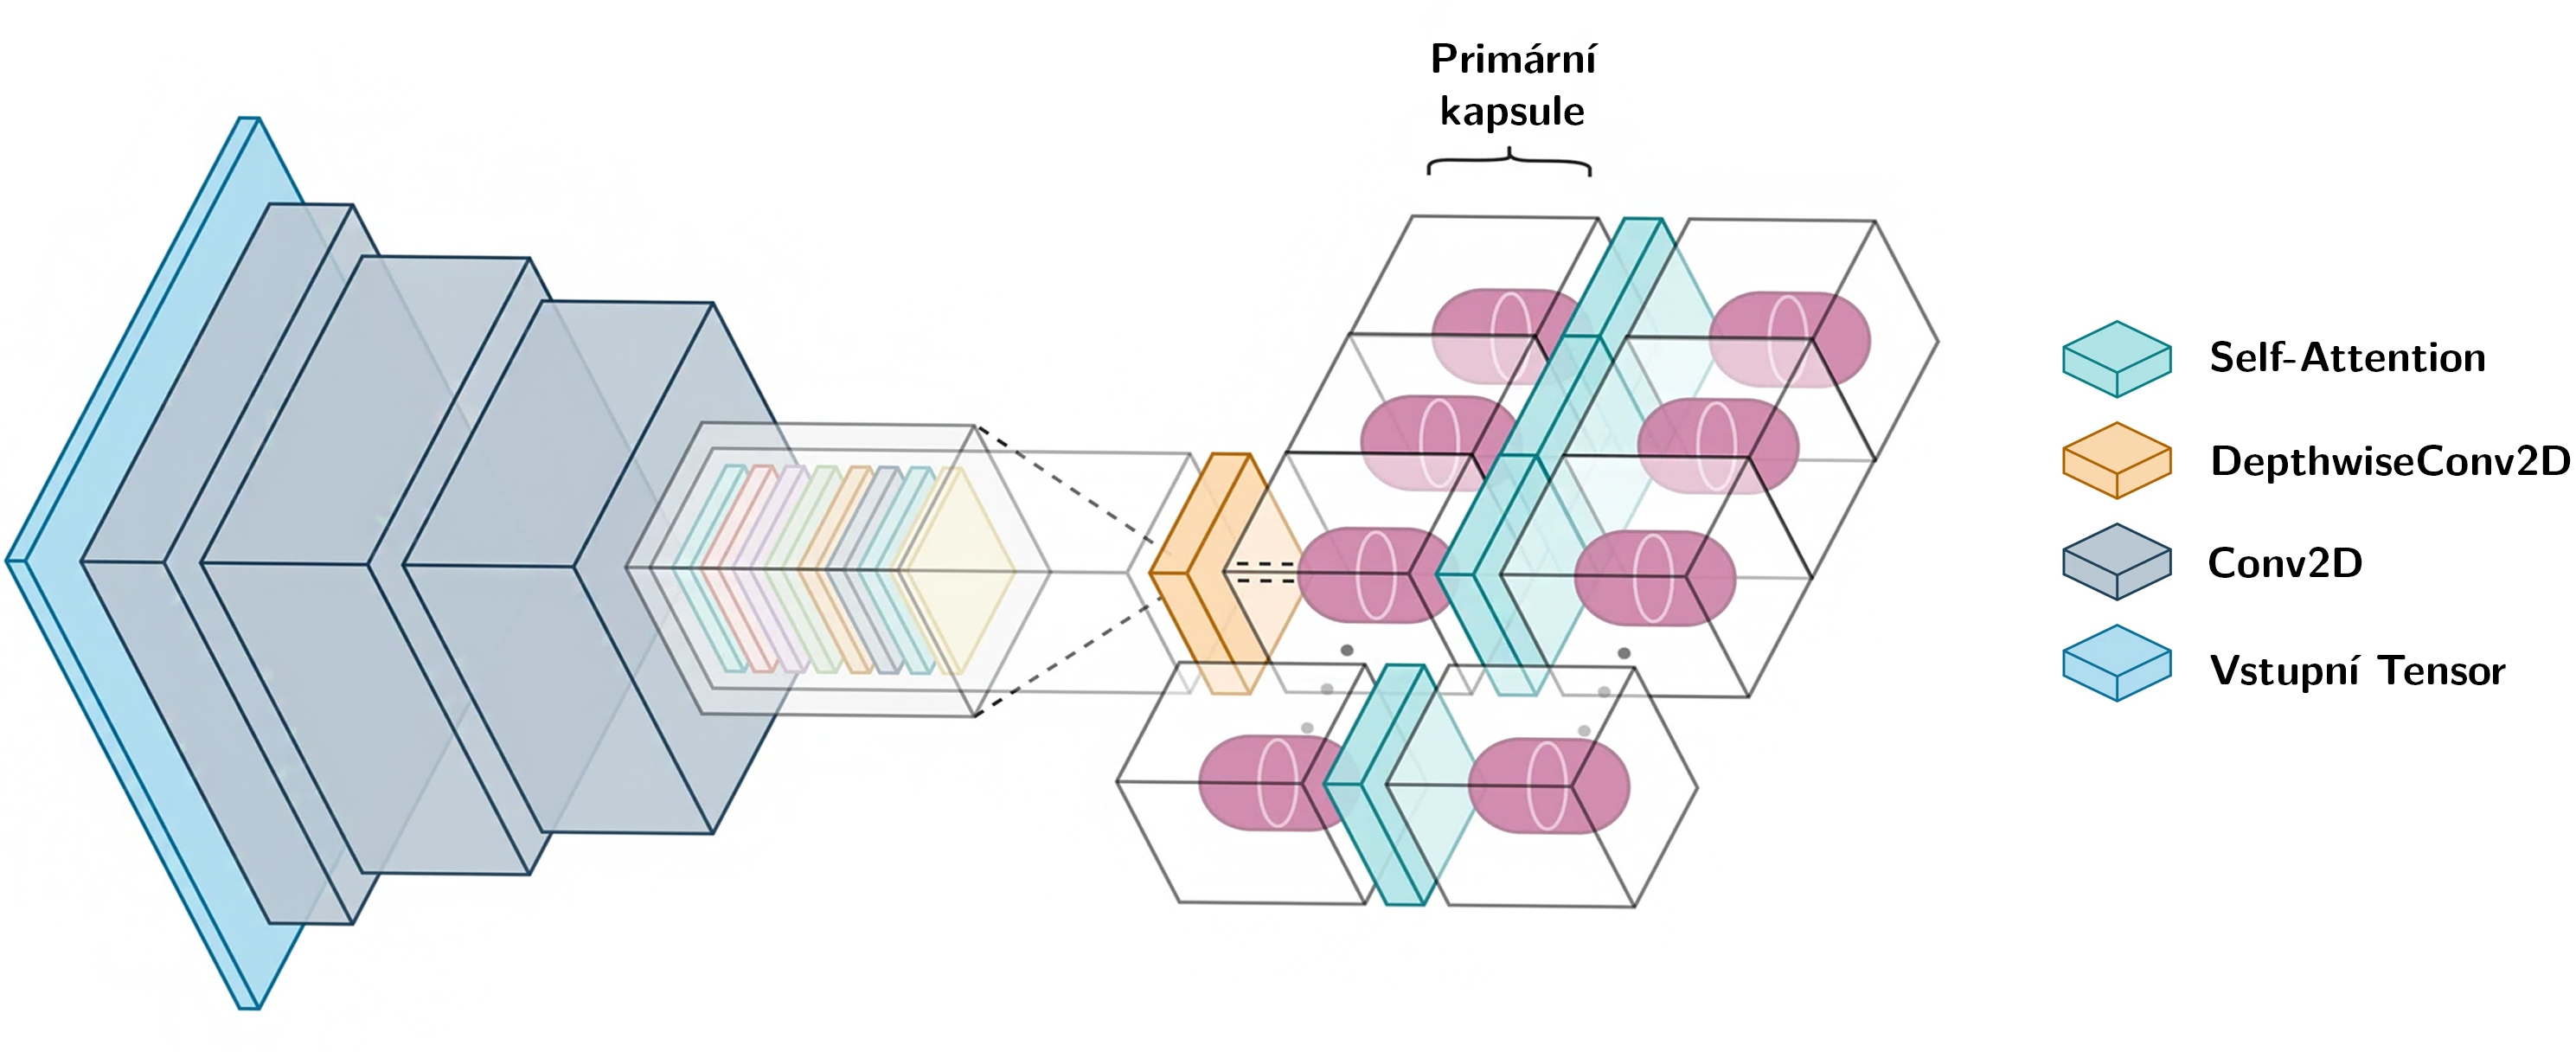
\includegraphics[width=1\linewidth]{figures/capsule}
        \caption{Schematické znázornění architektury sítě
            \textit{Efficient-CapsNet} (Upraveno a převzato z~\cite{Zhou2021})}
        \label{fig:architektura}
    \end{center}
\end{figure}

Zjednodušeně, v případě použití jednoho příznaku, je vstupem modelu obraz, který
lze reprezentovat jako tenzor $X$ s tvarem $H \times W \times C$, kde $H$, $W$ a
$C$ jsou výška, šířka a kanály. V našem případě se jedná o synergické spojení
dvou sad příznaků vyplývajících z minulých sekcí, kauzálních matic $X_{COG} \in
    \mathbb{R}^{T \times T \times C}$ a časoprostorových vzorů $X_{GAF} \in
    \mathbb{R}^{T \times T \times C}$. Vstupním tenzorem je tedy příznak $X \in
    \mathbb{R}^{2 \times T \times T \times C}$. Než se vstup dostane k primární
kapsulové vrstvě, tak je provedena extrakce lokálních vlastnosti ze vstupu $X$
pomocí sady několika typů vrstev\footnote{Jednotlivé vrstvy jsou pojmenovány
    podle korespondujícího názvu v \textit{TensorFlow} a \textit{Keras} API}:
\begin{itemize}
    \item \textbf{Conv2D} --- Tato vrstva vytváří konvoluční jádro, které je
          konvolvováno se vstupem vrstvy a vytváří tenzor výstupů. V podstatě se jedná
          o sadu naučitelných filtrů. Každý filtr transformuje část obrazu
          (definovanou velikostí jádra) pomocí filtru jádra. Matice jádrového filtru
          se aplikuje na celý obraz. Filtry lze chápat jako transformaci obrazu.
    \item \textbf{BatchNormalization} --- Tato vrstva aplikuje normalizaci,
          která udržuje průměrný výstup blízko nule a směrodatnou odchylku výstupu
          blízko jedné.
    \item \textbf{MaxPool2D} --- Tato vrstva funguje jednoduše jako filtr pro
          podvzorkování. Podívá se na 2 sousední pixely a vybere maximální hodnotu.
          Slouží ke snížení výpočetní náročnosti a do jisté míry také ke snížení
          přeučení.
    \item \textbf{Dropout} --- Dropout je regularizační metoda, při níž je část
          uzlů ve vrstvě náhodně ignorována (nastaveny na nulu) pro každý
          tréninkový vzorek. Tím se náhodně vynechá část sítě a síť je nucena
          učit se funkce distribuovaným způsobem. Tato technika také zlepšuje
          generalizaci a snižuje přeučení.
\end{itemize}

\begin{figure}[h]
    \begin{center}
        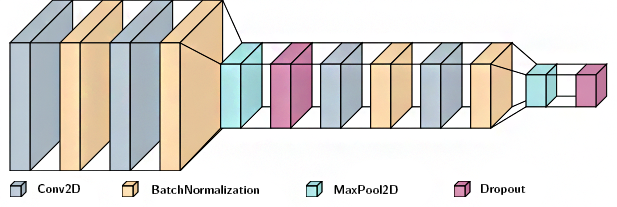
\includegraphics[width=0.85\linewidth]{figures/conv}
        \caption{První část sítě ($H_{Conv}$), která mapuje vstupní obraz na
            prostor vyšší dimenze}
        \label{fig:conv}
    \end{center}
\end{figure}

Každý výstup konvoluční vrstvy $l$ se tedy skládá z konvoluční operace s určitou
rozměrovou velikostí kernelů $k$ a počtem příznakových map $f$. U konvolučních
vrstev byla použita aktivační funkce $\operatorname{ReLU}$ k přidání nelinearity
do sítě:
\begin{equation}
    F^{l+1}\left(X^l\right)=\operatorname{ReLU}\left(\text {Conv}_{k \times k}\left(X^l\right)\right)
\end{equation}
Celkově si lze první část sítě představit jako jednu funkci $H_{Conv}$, která
mapuje vstupní obraz do prostoru s vyšší dimenzí, což usnadňuje tvorbu
kapslí\footnote{\enquote{Kapsle} označuje skupinu neuronů, která společně
představuje instanci parametru specifické entity nebo části obrazu}. Tuto první
část sítě lze vidět na Obr.~\ref{fig:conv}. Následně je pak využito hloubkově
oddělitelné konvoluce, ze které je získána vrstva primárních kapslí $S_{n,d}^l$
kde $n^l$ a $d^l$ jsou počty primárních kapslí a jejich jednotlivé rozměry
$l$-té vrstvy. Základním prvkem sítě tedy již není jeden neuron, ale vektorová
výstupní kapsle, která by měla zachovávat svojí orientaci a délku. To je
realizováno pomocí \enquote{\textit{squash}} aktivační funkce:
\begin{equation}
    \operatorname{squash}\left(s_n^l\right)=\left(1-\frac{1}{e^{\left\|s_n^l\right\|}}\right) \frac{s_n^l}{\left\|s_n^l\right\|}
\end{equation}
kde $s_n^l$ označuje právě jednu kapsli. Detailně koncept kapsulární sítě popsal
Hinton~\cite{Hinton2011}. Kapsulární neuronová síť byla implementována v
programovacím jazyce Python využitím knihoven
\textit{TensorFlow}\footnote{\url{https://www.tensorflow.org}} a
\textit{Keras}\footnote{\url{https://keras.io}}. Počet filtrů konvolučních
vrstev byl zvolen 32, 64, 64 a 128 v pořadí, tak jak jdou za sebou ve
schématu~\ref{fig:conv}. Velikosti kernelů byly zvoleny 5, 3, 3 a 3. MaxPool2D
vrstvy byly přidány k zajištění kombinace lokálních rysů příznaků a učení se tak
jeho globálnějším rysům. 

\subsection{Self-attention směrování}
\label{subsec:dynamicke_smerovani}
Kapsulární síť byla také v této práci zvolena, vzhledem k její architektuře
napodobující lidskou biologii, a tím pádem schopností lépe modelovat komplexní
vztahy v datech. To vyplývá z použitého nového přístupu neiterativního
paralelního směrování kapslí, které bylo představeno a popsáno
v~\cite{Mazzia2021}.

\subsection{Marginální ztrátová funkce}
\label{subsec:marginalni_funkce}
V případě této práce se jedná o binární klasifikační problém, pro který by se za
normálních okolností použila ztrátová funkce ve smyslu binární nebo kategorické
křížové entropie. Tyto ztrátové funkce ale nezachycují sémantiku vektorů, jak je
používána v kapslích. Pro tyto potřeby byla využita marginální ztrátová funkce,
kde v případě klasifikace více tříd, je pro každou třídu reprezentovanou kapslí
$n^L$ v poslední vrstvě $L$ vypočtena pravděpodobnost existence určité třídy
následovně:
\begin{equation}
    \mathcal{L}_{n^L}=T_{n^L} \max \left(0, m^{+}-\left\|u_n^L\right\|\right)^2+\lambda\left(1-T_{n^L}\right) \max \left(0,\left\|u_n^L\right\|-m^{-}\right)^2
\end{equation}
kde $T_{n^L}$ je rovno jedné, pokud je přítomna třída $n^L$, a $m^+$, $m^-$ a
$\lambda$ jsou laditelné hyperparametry. Nakonec jsou sečteny jednotlivé
ztrátové funkce $\mathcal{L}_{n^L}$ pro získání konečného \enquote{skóre} ve
fázi trénování.

\subsection{Trénování a evaluace modelů}
\label{subsec:trenovani_modelu}
Trénovaní a evaluace modelů bylo realizováno využitím programovacího jazyka
Python znovu ve spojení s interaktivním prostředím Jupyter Notebook. Pro tvorbu
modelů byly využity dříve zmíněné knihovny \textit{TensorFlow} a \textit{Keras}.
Trénování bylo akcelerováno pomocí grafické karty NVIDIA GeForce RTX 4080 s
využitím \textit{CUDA
Toolkitu}\footnote{\url{https://developer.nvidia.com/cuda-toolkit-archive}}
společně s \textit{CuDNN}\footnote{\url{https://developer.nvidia.com/cudnn}}
(NVIDIA CUDA® Deep Neural Network library) knihovnou. Pro účely trénování byly
datasety rozděleny vždy v poměru 8:2 na trénovací a testovací množinu, přičemž
validace probíhala během trénování využitím testovací množiny (resp. validační).
Všechny uvedené přesnosti ve výsledcích jsou tím pádem validační přesnosti,
nikoli trénovací. Pro trénování byl využit optimalizační algoritmus Adam s učící
rychlostí $5 \times 10^{-4}$. Trénování probíhalo po dobu 100 epoch a batch size
byl nastaven na 256. Pro zajištění rychlé konvergence optimalizátoru a co
nejblíže globálnímu minimu ztrátové funkce, byla použita metoda žíhání
(annealing) rychlosti učení (\gls{LR}, learning rate). Aby byla zachována výhoda
rychlého času výpočtu s vysokým \gls{LR}, byla dynamicky snižována \gls{LR}
každých $x$ kroků (epoch) v závislosti na tom, zda je to nutné (když se
nezlepšuje přesnost). Bylo také realizováno kombinační srovnání příznaků ve
smyslu použitých biosignálů. Veškeré výsledky jsou uvedeny v
sekci~\ref{sec:vysledky_detekce_cl}. Bylo realizováno i srovnání se současným
stavem. K evaluaci modelů byly využity hodnotící metriky, které jsou popsány v
sekci~\ref{subsec:ml_metriky}.